\documentclass[../main.tex]{subfiles}

\begin{document}
    \chapter{Experiments}\label{chap:experiments}

    \section{Implementation}\label{sec:implementation}
    We use Torch7 library~\cite{torch7} for implementation. The LoAd building blocks, besides the standard layers, are the
    element-wise multiplication and the depth contact operation, which are already available in Torch7.
    Regarding Grad-CAM, we start from the code provided by the authors~\cite{gradcam-github} and we modify it as discussed
    in Section~\ref{subsec:gradcam-domainness}.
    We implement the Spatial Pyramid Pooling layer as an extension of Torch7, and we build the computational graph to compose
    the building blocks into the overall end-to-end architecture.
    \newline\newline
    For each experiment setup, we train and test three different network configurations. All three variants starts from a baseline network pretrained on
    the \textit{ImageNet} dataset~\cite{imagenet}.
    In the first configuration (which we call Softmax), we replace only the last layer of the network with a new layer
    with dimension equal to the number of classes in the dataset. We train only this last layer, keeping all the other parameters frozen during training.
    In the second network (Spp), we remove all the fully-connected layers, as well as the last Max Pooling layer.
    We replace the latter with a Spatial Pyramid Pooling layer, and we add new fully-connected layers on top of it.
    The third network is LoAd, whom architecture is discussed in Section~\ref{sec:load-network}. Note that in Spp and LoAd the substitution of
    the fully-connected layers is necessary, as in a feed-forward network the removal of layer $i$ constrains us to remove also layers $i + 1$ to $n$.
    \\
    With this configuration of networks, we are able to verify the
    effectiveness of each component of the LoAd Network. In one experiment setting, we also compare our technique
    against state-of-the-art approaches.

    \section{Experiment settings}

    \subsection{Baseline Networks}\label{subsec:networks}
    In our experiments we use two baseline networks. The first is \textit{Alexnet}~\cite{alexnet}, winner of the ILSVRC 2012 competition
    and the responsible for the recent deep learning revolution in computer vision. The paper introduced many interesting innovations, most
    notably the use of Graphics Processing Units (GPUs) to train neural networks with millions of parameters at large scale, a method
    to reduce overfitting known as Dropout, and the use of the Rectified Linear Unit (ReLU) activation function.
    The second network is VGG16~\cite{vgg16}, winner of the ILSVRC 2014 competition.
    VGG16 is much deeper than Alexnet, in fact Alexnet has 5 convolutional layers and 3 fully-connected layers, while VGG16 has 13
    convolutional layers and 3 fully-connected layers. The use of two baseline networks improves the reliability of our findings.

    \subsection{Training procedure}
    Each network is trained using the same set of hyperparameters, established by using a validation set to search over a grid of
    possible values.
    The parameters of the first $f$ layers are frozen, where $f = 22$ for AlexNet (Softmax), $f = 38$ for VGG16 (Softmax),
    $f = 5$ for AlexNet (Spp and LoAd), $f = 12$ for VGG16 (Spp and LoAd).
    The parameters of layers $f + 1$ to $g$ are not frozen, but they are set with a small learning rate $\alpha_{f+1,g} = 10^{-5}$ (Spp and LoAd)
    and $\alpha_{f+1,g} = 0$ (Softmax). $g$ is the number of layers that are retained from the ImageNet baseline.
    The parameters of layers $g + 1$ to $n$ have a higher learning rate $\alpha_{g+1,n} = 10^{-3}$ (Softmax) and $\alpha_{g+1,n} = 5 \times 10^{-4}$
    (Spp and LoAd). Also, for all the layers that are trained from random initialization, a weight decay of $w = 5 \times 10^{-4}$ is used as a regularizer.
    In Spp and LoAd, fully-connected layers have dimension $2048 \rightarrow 2048 \rightarrow 15 $ for AlexNet and $4096 \rightarrow 2048
    \rightarrow 15 $ for VGG16, and they uses dropout with $p = 0.6$.

    The optimizer used in the training procedure is Stochastic Gradient Descent with Momentum~\cite{momentum}. The momentum parameter
    is set to 0.9, with nesterov momentum~\cite{nesterov-momentum} enabled.
    We use a batch size of 256 for AlexNet and 16 for VGG16 (due to the high memory footprint of this network).
    Training was performed in parallel on multiple NVIDIA Titan X GPUs.

    \subsection{Datasets and Metrics}
    We evaluate our LoAd on two variants of the iCub World dataset~\cite{icw}, which we call respectively iCW-translation and iCW-scale.
    Both datasets have two domains. As the names suggest, in the former case the shift between the two domains is caused by large
    object translations, while in the latter it is caused by scale variations. It is worth noting that, as discussed in Section~\ref{subsec:convnets},
    CNNs are known to handle some degree of scale and translation invariances. However, using a network structure specifically designed
    to handle such invariances have been shown to be more successful in many tasks~\cite{sppooling}. 
    In both datasets, one domain is composed by 4500 images and the other one by 3000 images. These are rather small
    datasets for data-hungry deep learning models, hence the choice of starting from ImageNet baselines.
    For iCW-translation, we also compare against prior state-of-the-art approaches.
    \newline\newline
    To measure performance, we train each network over one domain and use the other domain as the test set, measuring
    classification accuracy. In order to improve statistical robustness, we run all the
    experiments 5 times, and we report mean and standard deviation of the results.

    \subsection{The iCub World dataset}
    The iCW Transformations dataset~\cite{icw} contains images with objects from 15 categories, acquired through a robot camera.
    Each object is acquired while undergoing isolated visual transformations, in order to study invariance to real-world nuisances.
    A human operator moves the object holding it in the hand and the robot tracks it by exploiting either motion cues or depth cues.
    Different datasets are available depending on the object transformation carried out by the human.
    We will use two different variants of the iCW Transformations dataset:

    \begin{itemize}
        \item \textbf{Translation}: The human moves in a semi-circle around the iCub robot, keeping approximately the same
            distance and pose of the object in the hand with respect to the cameras. We use only images taken at the extreme of the
            semi-circle, thus the object appears either at the left of the image or at the right. Another cause of domain shift is
            that the background changes dramatically, while the object appearance remains the same.
        \item \textbf{Scaling}: The human moves the hand holding the object back and forth, thus changing the object's
            scale with respect to the cameras. In this case the two domains are again defined by keeping the images at the extreme of
            the object movement: far or close to the camera.
    \end{itemize}

    For each of the two variations the classes are perfectly balanced, namely each one has the same number of samples. Each dataset
    has two domains, which are both in turn considered as source and target.
    In figure~\ref{fig:icw-samples}, we can see a random sample of images from the dataset.

    \begin{figure}[h!]
        \centering{}
        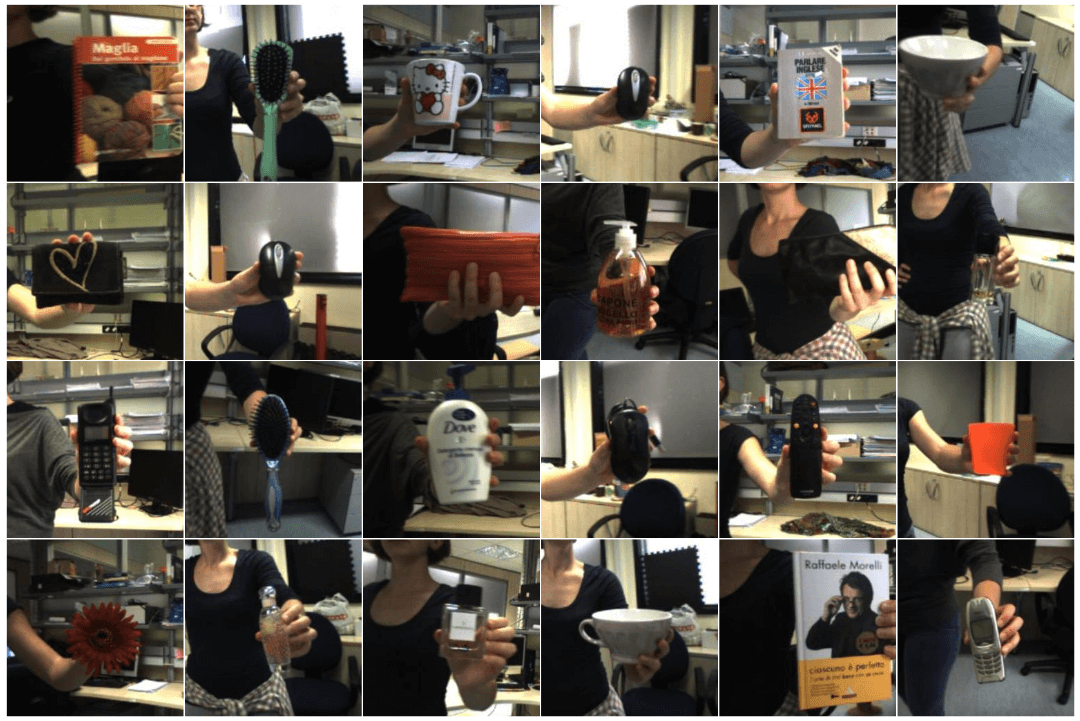
\includegraphics[width=\linewidth]{./img/icw-samples.png}
        \caption{Random sample from the iCubWorld dataset.}\label{fig:icw-samples}
    \end{figure}

    \paragraph{Domain Shift}
    The first thing to do is to verify if the iCW dataset actually represents a domain adaptation task. That is,
    we should measure the domain shift in the dataset. In the domain adaptation literature, this is usually
    done in the following way: we train a classifier on 80\% of the source domain, and we test it both on the
    remaining 20\% and on the target domain. The absolute difference of performance gives a
    rough quantitative measure of the domain shift. Intuitively, the more the performance difference,
    the more the two datasets were generated from different distributions. The following process is employed
    to measure this domain shift. First, image features are extracted at the second fully-connected layer of the
    VGG16. This gives a feature vector of 4096 entries for each image. We then run a Linear Support Vector Machine
    classifier~\cite{fan2008liblinear} on top of these features. Results for both iCW translation and iCW scale
	are shown in Table~\ref{table:domain-shift}.

	\begin{table}[!ht]
		\centering{}
		\begin{tabular}{l c c c}
			\toprule
                     & S (80\%) $\rightarrow$ S (20\%)  & S (80\%) $\rightarrow$ T & Difference \\
			\midrule
			Left 1 $\rightarrow$ Left 2   & 99.67  & 59.23 & 40.44 \\
			Left 2 $\rightarrow$ Left 1   & 99.83  & 62.47 & 37.36 \\
			Scale 1 $\rightarrow$ Scale 2 & 100.00 & 26.54 & 73.46 \\
			Scale 2 $\rightarrow$ Scale 1 & 99.67  & 40.98 & 58.69 \\

		\end{tabular}
		\caption{iCW domain shift measure.~\textit{S} stands for Source.~\textit{T} stands for Target. \textit{X} $\rightarrow$ \textit{Y} means that the SVM is trained on \texit{X} and tested on \textit{Y}.}\label{table:domain-shift}
	\end{table}

	In both datasets, there is a clear domain shift between the two domains. Also, by looking at Table~\ref{table:domain-shift},
	we can also see for instance that the task Scale 1 $\rightarrow$ Scale 2 is much more difficult than the opposite one. This
	might be because Scale 2 images contains information that helps the classifier also on Scale 1, but the opposite is not true.

	Having seen that there is indeed a domain shift between the domains, in the next paragraph we compare our method both with
	standard transfer learning techniques and with the state-of-the-art Domain-Adversarial Networks~\cite{DANN}.

    \subsubsection{Results}\label{subsubsec:results}
	In the following tables we report the results of our experiments. In particular, we report the percentage of classification accuracy:
    the fraction of correctly annotated samples over the total cardinality of the target set.
    We can see that our method LoAd outperforms
	all the other techniques by a significant margin.
    \newline

    \begin{table}[!ht]
        \centering{}
        \begin{tabular}{l c c c}
            \toprule
                     & Left 1 $\rightarrow$ Left 2 & Left 2 $\rightarrow$ Left 1 & Average \\
            \midrule
            Softmax  & $50.41 \pm{} 0.98$ & $54.01 \pm{} 0.59$ & 52.21 \\
            Spp      & $63.55 \pm{} 1.49$ & $61.15 \pm{} 0.69$ & 62.35 \\
            DANN     &  63.20             &  42.93             & 53.07 \\
        \textbf{LoAd} & $\mathbf{67.35 \pm{} 0.97}$ & $\mathbf{61.75 \pm{} 0.54}$ & \textbf{64.55} \\
            \bottomrule
        \end{tabular}
        \caption{iCW Translation Alexnet Results.}
    \end{table}

    \begin{table}[!ht]
        \centering{}
        \begin{tabular}{l c c c}
            \toprule
                     & Left 1 $\rightarrow$ Left2 & Left 2 $\rightarrow$ Left 1 & Average \\
            \midrule
            Softmax  & $62.15 \pm{} 0.94$ & $64.74 \pm{} 0.92$ & 63.44 \\
            Spp      & $75.14 \pm{} 1.09$ & $75.91 \pm{} 1.26$ & 75.53 \\
            DANN     &  76.43             &  54.60             & 65.52 \\
        \textbf{LoAd} & $\mathbf{78.17 \pm{} 0.66}$ & $\mathbf{77.30 \pm{} 0.80}$ & \textbf{77.73} \\
            \bottomrule
        \end{tabular}
        \caption{iCW Translation VGG16 Results.}
    \end{table}

    \begin{table}[!ht]
        \centering{}
        \begin{tabular}{l c c c}
            \toprule
                     & Left 1 $\rightarrow$ Left2 & Left 2 $\rightarrow$ Left 1 & Average \\
            \midrule
            Softmax  & $18.20 \pm{} 0.71$ & $27.45 \pm{} 1.23$ & 22.83 \\
            Spp      & $25.77 \pm{} 0.88$ & $30.52 \pm{} 0.60$ & 28.15 \\
        \textbf{LoAd} & $\mathbf{29.68 \pm{} 1.52}$ & $\mathbf{31.43 \pm{} 0.49}$ & \textbf{30.56} \\
            \bottomrule
        \end{tabular}
        \caption{iCW Scale Alexnet Results.}
    \end{table}
    
    \begin{table}[!ht]
        \centering{}
        \begin{tabular}{l c c c}
            \toprule
                     & Left 1 $\rightarrow$ Left 2 & Left 2 $\rightarrow$ Left 1 & Average \\
            \midrule
            Softmax  & $30.85 \pm{} 0.67$ & $49.88 \pm{} 0.73$ & 40.36 \\
            Spp      & $35.69 \pm{} 1.08$ & $49.85 \pm{} 1.38$ & 42.77 \\
        \textbf{LoAd} & $\mathbf{42.16 \pm{} 1.09}$ & $\mathbf{50.69 \pm{} 0.96}$ & \textbf{46.42} \\
            \bottomrule
        \end{tabular}
        \caption{iCW Scale VGG16 Results.}
    \end{table}
    
    Besides observing the final classification accuracy of our LoAd network, we also verified that the features
    learned with our architecture are more robust to domain shift than that obtained through standard CNN without
    adaptation. Namely, we train a binary classifier to tell which distribution (source or target) samples were drawn from.
    Intuitively, if the distributions are the same, we should expect a classification accuracy of $\sim 50\%$,
    whether if the distributios are different, we should expect an accuracy of $\sim 100\%$.
    This is indeed the case, as we've verified experimentally. What we would like to verify however, is if
    LoAd actually reduces the performance of such a binary classifier. 

    \begin{table}[!ht]
        \centering{}
        \begin{tabular}{l c c}
            \toprule
            & iCW Translation & iCW Scale \\
            \midrule
            ImageNet & 96.67 & 97.87 \\
            Softmax  & 98.87 & 99.20 \\
        \textbf{LoAd} & $\mathbf{93.03}$ & $\mathbf{95.28}$ \\
            \bottomrule
        \end{tabular}
        \caption{Domain shift reduction caused by LoAd\@. The binary classifier is a Linear SVM trained on top of
        features extracted from VGG16. Lower is better.}\label{table:domain-shift-LoAd}
    \end{table}
    
    As the results in Table~\ref{table:domain-shift-LoAd}
    shows, LoAd actually reduces the performance of the classifier (albeit by a little amount), hence making the
    two distributions more similar.

\end{document}
